\section{(Alternate) Predicting ELMs in novel sequences}
\label{sec:predicting_cv_0974}

TODO: DESCRIBE MOST PROBABLE MOTIF INSTANCES (COMPARED TO FILTERED)

We will use protein \uniprot{CV\_0974} (uniprot ID: Q7NZE8) as an example, a
``probable tyrosine phosphatase'' from \emph{Chromobacterium violaceum}.
This protein is predicted to be a tyrosine phosphates because it has a
``tyrosine phosphatase'' (PTPc) domain.

%
% Subsection: Necessary Resources
%
\subsection{Necessary Resources}

\subsubsection{Software \& Hardware}

A modern browser such as Firefox, Chrome, Safari. ELM is best viewed on
a laptop or desktop computer, although tablets and smartphones will also
work.

\begin{enumerate}

%
% Subsection: Submitting a query
%
\subsection{Submitting a query to ELM}
\label{subsec:predicting_cv_0974_submitting}

\begin{figure}[h!]
	\centering
	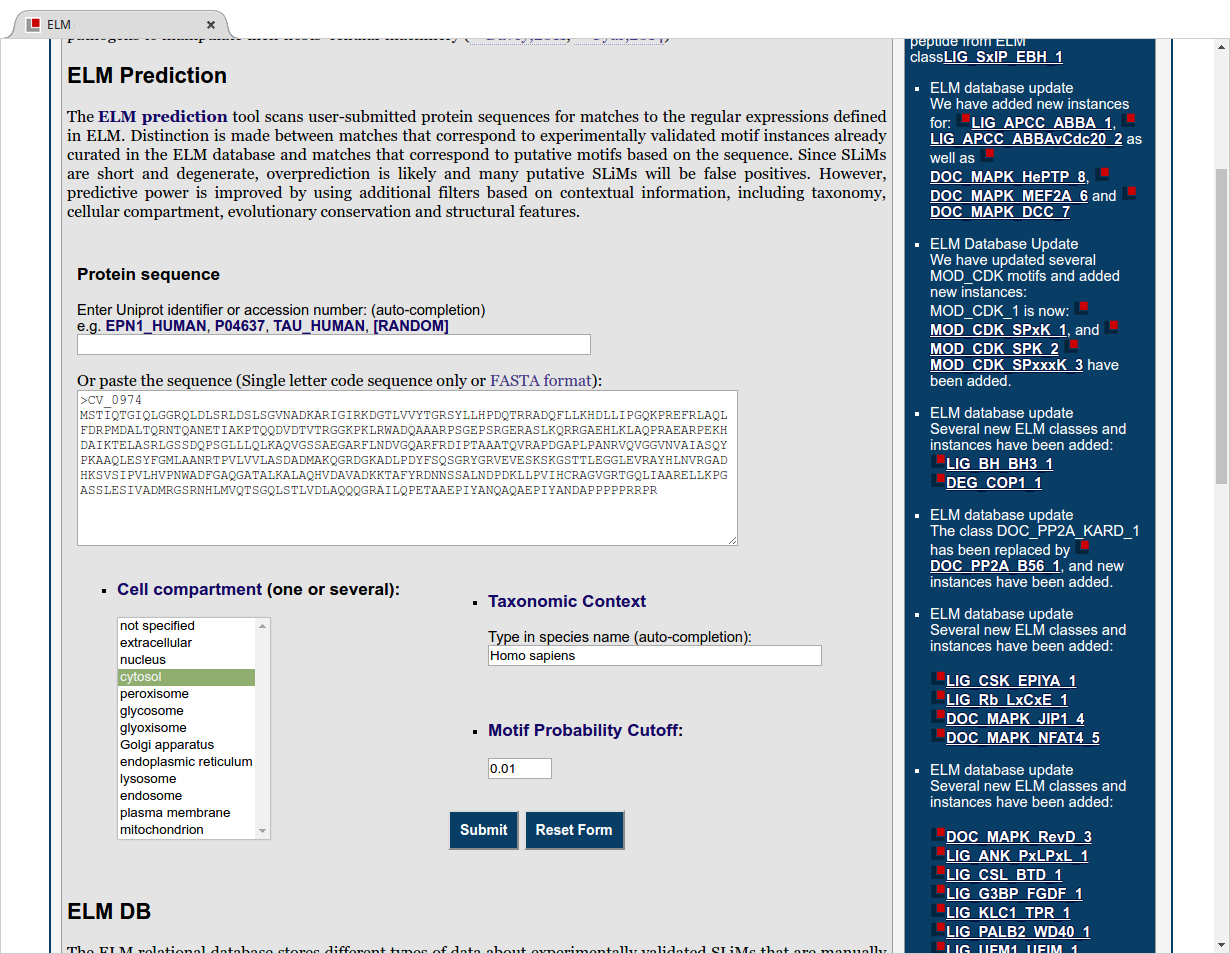
\includegraphics[width=\textwidth]{Figures/predicting_cv_0974/elm_search.png} 
	\caption{
	\textbf{Figure BACT-BP-1:}
	The input query page for finding motifs in ELM. The sequence
	for \emph{C. vilaceum protein} CV\_0974 was used as an example for this
	protocol.
	}
	\label{fig:predicting_cv_0974_search}
\end{figure}

\item Click on the ``ELM Predictions'' button in the menu to access the search
	query page (Fig. \ref{fig:predicting_cv_0974_search}).
	Here you can provide either a protein
	accession (from uniprot) or an amino acid sequence (simply the
	sequence, or a FASTA formatted entry) in which you want to detect
	SLiMs.  Retrieve the FASTA formatted sequence from Uniprot
	(http://www.uniprot.org/uniprot/Q7NZE8.fasta), and enter it into the
	``sequence input text box''.

TODO: MENTION NOT TO USE ``CHROMOBACTERIUM VIOLACEUM'' IN THE ORGANISM
BOX AND WHY

\begin{figure}[h!]
	\centering
	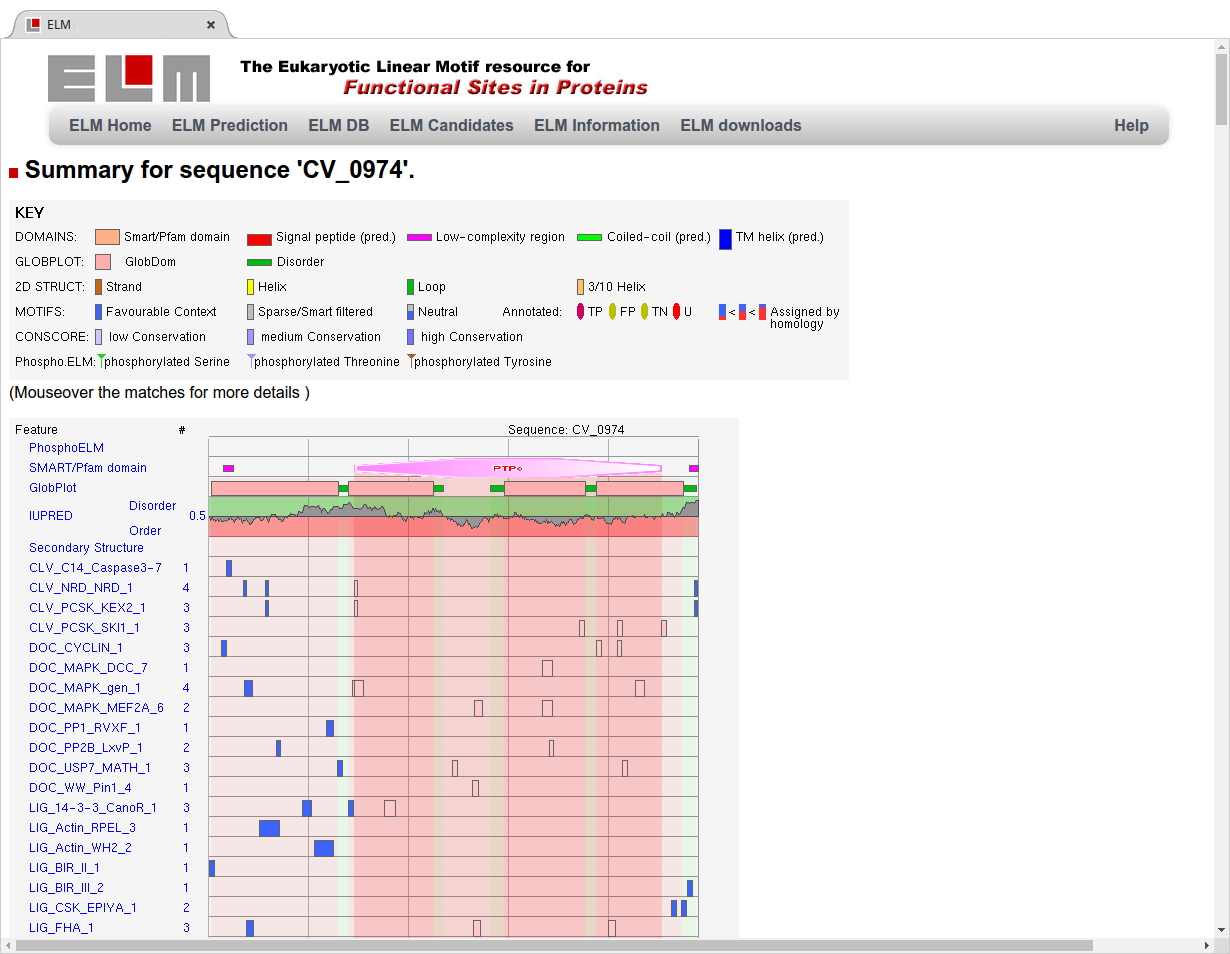
\includegraphics[width=\textwidth]{Figures/predicting_cv_0974/elm_results_summary.png}
	\caption{
	\textbf{Figure BACT-BP-2:}
	The graphical results summary of the ELM Prediction pipeline for
	Probable Tyrosine phosphate (CV\_0974). Note that not all motif
	detections are shown (the image is truncated at the bottom). The top
	five rows show a handfull of structural features. The motif occurence
	are shown as blue boxes, the intensity of which indicates the
	conservation score. See steps XXX to YYY for more information.
	}
	\label{fig:predicting_cv_0974_results_summary}
\end{figure}

\item The Results are summarized in the first figure on the results page
	(see Fig. \ref{fig:predicting_cv_0974_results_summary})
	The Graphical summary shows all of the final and
	intermediate results generated by the ELM Prediction pipeline, and can
	be used infer whether or not a motif is present in a sequence, as well
	as now likely it is to be functional based on its structural context
	and evolutionary conservation.

\item Check the first row to see whether there are for phosphorylation sites
	acid is a serine, threonine or tyrosine. In this case, no
	phosphorylation data could be found in the Phospho.ELM database
	(\cite{21062810}).

\item Check the second row showing SMART and Pfam domains. Hover the mouse over
	these domains to see their names and exact start and end positions.

\item The third row shows globular and disordered regions in the sequence as
	predicted by GlobPlot (\cite{12824398}). The 4th \& 5th rows contain
	results from IUPred (\cite{15955779}), another unstructured region
	prediction tool. Protein segments with an IUpred score above 0.5 are
	95\% likely to be disorered (REF???).  

\item Place the cursor over the blue box for motif occurence
	``DOC\_USP7\_MATH\_1'' at position 129-133. This motif is in a
	disorered region, and has not been filtered out by the structural
	filter. However, its conservation score is extremely low: 0.000,
	indicating it is not conserved in homologous proteins. Place the cursor
	over motif ``DOC\_MAPK\_DCC\_7'' at positions ``334-343''. Despite the
	high conservation score (1.000), this motif is inside the PTPc domain
	(and a Globular regions), and therefore has been filtered out.

TODO: CHECK CONSERVATION FILTER

%
% Subsection: Submitting a query
%
\subsection{Interpreting the prediction results: Additional Information}
\label{subsec:predicting_cv_0974_additional_information}

TODO: DESCRIBE HOW TO INTERPRETE THE PREDICTIONS USING THIS BACTERIAL
EXAMPLE (OF WHICH NOT MUCH IS KNOWN). FOCUS ON HOW ONE SHOULD INTERPRETE
THESE PREDICTIONS (LOOK AT DISORDER/GLOBULARITY, CONSERVATION)

\end{enumerate}
